% Part: sets-functions-relations
% Chapter: relations
% Section: graphs

\documentclass[../../../include/open-logic-section]{subfiles}

\begin{document}

\olfileid{sfr}{rel}{grp}
\olsection{ګرافونه}

\emph{ګراف} داسې شکل دے چې ټکي—چې ``غوټې'' يا ``څوکې'' (د
``څوکه'' جمع) بللے شي—پکښې د څنډو په ذريعه سره نښتي وي۔ ګرافونه
په منفصل رياضي او کمپيوټرپوهنه کښې هر ځاے کارېدونکې وسيلې دي۔
د اړيکو او جوړښتونو د ښودلو او انځورولو دپاره ډېر ګټور دي؛ له
محسوسو څيزونو، لکه د بېلو ډولونو له شبکو، نيولې تر مجردو جوړښتونو،
لکه د پرېکړو تر ممکنو پايلو پورې۔ په علمي ليکنو کښې د ګرافونو ډېر
بېل ډولونه شته۔ مثلاً، په دې سره توپير کوي چې څنډې لوری لري که نه،
نوم نښې لري که نه، آيا له يوې غوټې بېرته هماغې غوټې ته څنډې کېدلے
شي، د هماغو غوټو ترمنځ څو څنډې کېدلے شي، او داسې نور۔
\emph{لوری لرونکي ګرافونه} له اړيکو سره يو خاص تړاو لري۔

\begin{defn}[لوری لرونکے ګراف]
\emph{لوری لرونکے ګراف} $G = \tuple{V, E}$ د \emph{څوکو} يو سټ
$V$ او د \emph{څنډو} يو سټ $E \subseteq V^2$ دے۔
\end{defn}

\begin{explain}
زمونږ د تعريف له مخې، ګراف يوازې يو سټ او په همدغه سټ باندې يوه
اړيکه ده۔ البته، د ګرافونو په اړه د خبرو پر وخت، په شکل کښې د
ښودلو تمه ئې طبيعي ده: ګراف داسې رسمولے شو چې دوه څوکې $v_1$ او
$v_2$ په يو غشي هله او يوازې هله سره ونښلوو چې
$\tuple{v_1, v_2} \in E$ وي۔ د يوازې اړيکې او ګراف ترمنځ توپير
يوازې دا دے چې ګراف د څوکو سټ ټاکي؛ يعنې ګراف ګوښې څوکې هم
لرلے شي۔ خو مهمه خبره دا ده چې په سټ $X$ باندې هره اړيکه $R$ د
يو لوری لرونکي ګراف $\tuple{X, R}$ په توګه کتلے شو۔ برعکس، يو
لوری لرونکے ګراف $\tuple{V, E}$ د اړيکې $E \subseteq V^2$ په
توګه کتلے شو چې سټ $V$ پکښې په څرګنده ټاکل شوے وي۔
\end{explain}

\begin{ex}
هغه ګراف $\tuple{V, E}$ چې
$V = \{1, 2, 3, 4\}$ او
$E = \{\tuple{1,1}, \allowbreak \tuple{1, 2}, \allowbreak \tuple{1, 3},
\allowbreak \tuple{2, 3}\}$ وي، داسې ښکاري:
\begin{align*}
& 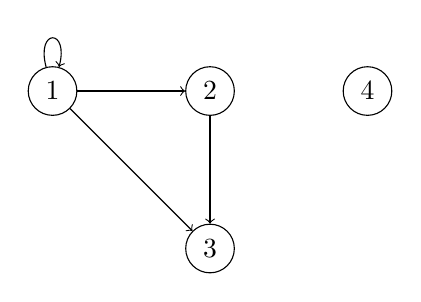
\begin{tikzpicture}[->,node distance=2cm]
  \node[draw,circle] (A) {$1$};
  \node[draw,circle] (B) [right of=A] {$2$};
  \node[draw,circle] (C) [below of=B] {$3$};
  \node[draw,circle] (D) [right of=B] {$4$};
  \draw (A) to [loop above]  (A);
  \draw (A) to  (B);
  \draw (A) to  (C);
  \draw (B) to  (C);
  \end{tikzpicture}
\intertext{دا له هغه ګراف $\tuple{V', E}$ څخه بېل دے چې
  $V' = \{1, 2, 3\}$ وي، او داسې ښکاري:}
& 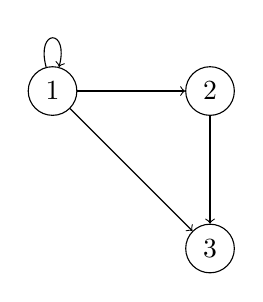
\begin{tikzpicture}[->,node distance=2cm]
  \node[draw,circle] (A) {$1$};
  \node[draw,circle] (B) [right of=A] {$2$};
  \node[draw,circle] (C) [below of=B] {$3$};
  \draw (A) to [loop above]  (A);
  \draw (A) to  (B);
  \draw (A) to  (C);
  \draw (B) to  (C);
  \end{tikzpicture}
\end{align*}
\end{ex}

\begin{prob}
  په سټ $\{1, 2, 3, 4\}$ باندې د کوچني يا برابر کېدو اړيکه
  $\le$ د ګراف په توګه وګورئ او ورسره سم شکل رسم کړئ۔
\end{prob}

\end{document}
